% Options for packages loaded elsewhere
\PassOptionsToPackage{unicode}{hyperref}
\PassOptionsToPackage{hyphens}{url}
%
\documentclass[
]{article}
\usepackage{amsmath,amssymb}
\usepackage{lmodern}
\usepackage{iftex}
\ifPDFTeX
  \usepackage[T1]{fontenc}
  \usepackage[utf8]{inputenc}
  \usepackage{textcomp} % provide euro and other symbols
\else % if luatex or xetex
  \usepackage{unicode-math}
  \defaultfontfeatures{Scale=MatchLowercase}
  \defaultfontfeatures[\rmfamily]{Ligatures=TeX,Scale=1}
\fi
% Use upquote if available, for straight quotes in verbatim environments
\IfFileExists{upquote.sty}{\usepackage{upquote}}{}
\IfFileExists{microtype.sty}{% use microtype if available
  \usepackage[]{microtype}
  \UseMicrotypeSet[protrusion]{basicmath} % disable protrusion for tt fonts
}{}
\makeatletter
\@ifundefined{KOMAClassName}{% if non-KOMA class
  \IfFileExists{parskip.sty}{%
    \usepackage{parskip}
  }{% else
    \setlength{\parindent}{0pt}
    \setlength{\parskip}{6pt plus 2pt minus 1pt}}
}{% if KOMA class
  \KOMAoptions{parskip=half}}
\makeatother
\usepackage{xcolor}
\usepackage[margin=1in]{geometry}
\usepackage{graphicx}
\makeatletter
\def\maxwidth{\ifdim\Gin@nat@width>\linewidth\linewidth\else\Gin@nat@width\fi}
\def\maxheight{\ifdim\Gin@nat@height>\textheight\textheight\else\Gin@nat@height\fi}
\makeatother
% Scale images if necessary, so that they will not overflow the page
% margins by default, and it is still possible to overwrite the defaults
% using explicit options in \includegraphics[width, height, ...]{}
\setkeys{Gin}{width=\maxwidth,height=\maxheight,keepaspectratio}
% Set default figure placement to htbp
\makeatletter
\def\fps@figure{htbp}
\makeatother
\setlength{\emergencystretch}{3em} % prevent overfull lines
\providecommand{\tightlist}{%
  \setlength{\itemsep}{0pt}\setlength{\parskip}{0pt}}
\setcounter{secnumdepth}{5}
\usepackage{amsmath}
\usepackage{amssymb}
\usepackage{float}
\usepackage{titling}
\usepackage[
backend=biber,
natbib=true,
language = english,
doi = false, url = false, isbn = false, eprint = false,
style = apa]
{biblatex}
\usepackage{xcolor}
\ifLuaTeX
  \usepackage{selnolig}  % disable illegal ligatures
\fi
\IfFileExists{bookmark.sty}{\usepackage{bookmark}}{\usepackage{hyperref}}
\IfFileExists{xurl.sty}{\usepackage{xurl}}{} % add URL line breaks if available
\urlstyle{same} % disable monospaced font for URLs
\hypersetup{
  pdfauthor={Group II},
  hidelinks,
  pdfcreator={LaTeX via pandoc}}

\DeclareLanguageMapping{english}{english-apa}
\addbibresource{literature.bib}

\title{The Price Air Pollution\\
1436 - Spatial Economics}
\author{Group II}
\date{12/31/2022}

\begin{document}
\maketitle

\begin{center}
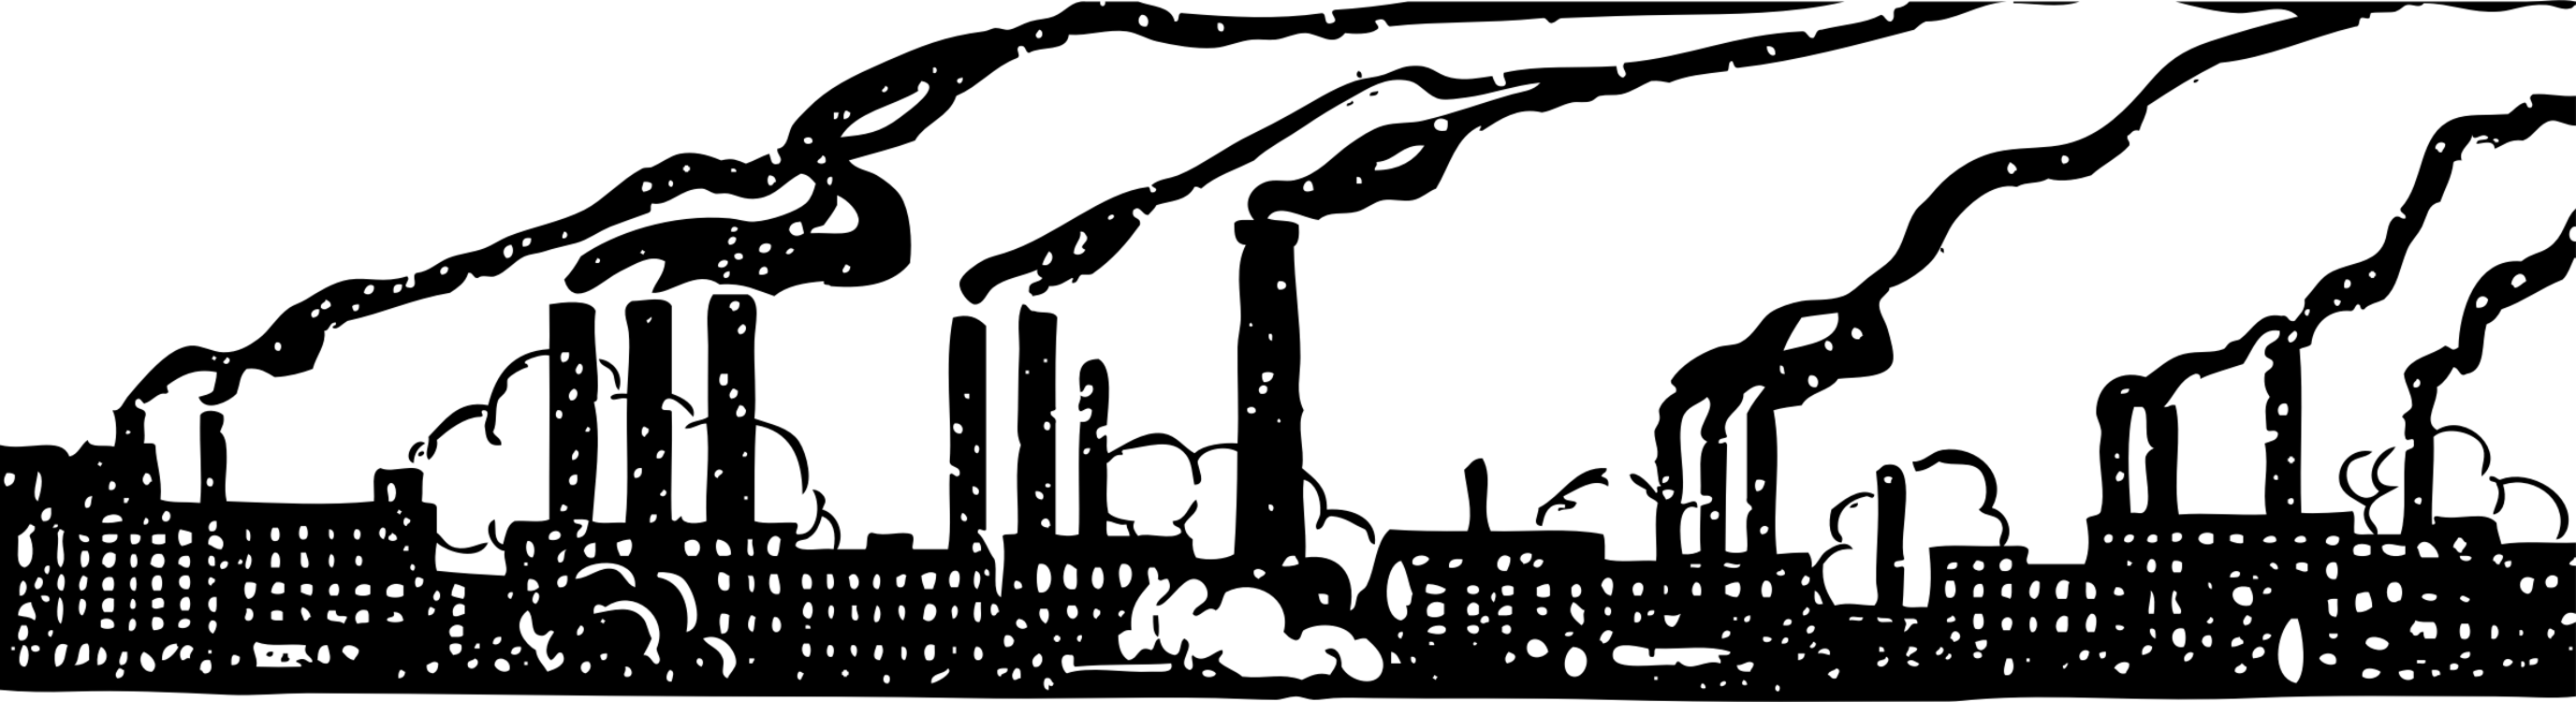
\includegraphics[width = 380pt]{pollution.png} 
\end{center}
\thispagestyle{empty}
\newpage
\pagenumbering{arabic}

\hypertarget{introduction}{%
\section{Introduction}\label{introduction}}

In 2019 the major premature death causes in China were cardiovascular diseases totaling 43 percent, followed by malignant neoplasms (26 percent), respiratory diseases (10 percent), unintentional injuries (6 percent) and neurological conditions (4 percent). Other conditions that accounted for between 3 and 1 percent of premature deaths, in descending order, were digestive diseases, genitourinary diseases, respiratory infections, diabetes mellitus and infectious and parasitic diseases. %https://www.who.int/data/gho/data/themes/mortality-and-global-health-estimates/ghe-leading-causes-of-death

\hypertarget{literature review}{%
\section{Literature review}\label{Literature review}}

\subsection{Effects of air pollution on health}

Analysing the effect of air pollution on health expenditures implicitly implies the aforementioned causal transition dependencies. Various studies have identified direct effects of exposure to air pollution on health. %(Quellen einfügen bei "various studies")

Franklin, Brook, Pope III (2015) and Fiordelisi et al. (2017) demonstrate that the risk of cardiovascular diseases and the triggering of acute cardiac events is increased by PM air pollution. The pathways through which this occurs include the generation of proinflammatory or oxidative stress mediators in the lung that enter the systemic circulation, the direct infiltration of certain particles or components into the cardiovascular tissue, or an imbalance of the autonomous nervous system. In that context, Hoek et. al (2013) quantify the effect of PM2,5 long-term exposure by conducting a meta-analytic review of previous studies. Their pooled estimate indicates an increase in all-cause mortality and cardiovascular mortality of 6 percent and 11 percent, respectively, if increments of PM2,5 are increased by 10-myg/m3. Equivalently, an increase in NO concentration of the same magnitude leads to an increased all-cause mortality of five percent. %https://www.sciencedirect.com/science/article/pii/S0146280615000043; https://ehjournal.biomedcentral.com/articles/10.1186/1476-069X-12-43; https://pubmed.ncbi.nlm.nih.gov/28303426/

tbd Respiratory diseases %https://www.ncbi.nlm.nih.gov/pmc/articles/PMC6033955/
tbd lung cancer %https://www.jstor.org/stable/3703988

tbd DALY %https://www.nature.com/articles/nature15371; https://www.sciencedirect.com/science/article/pii/S0140673616315975?ref=cra_js_challenge&fr=RR-1

Additionally, Zhao et al. suggest that based on recent findings air pollution may be involved in the development of autoimmune diseases such as diabetes mellitus, multiple sclerosis, or rheumatoid arthritis. The authors argue that air pollution can cause imbalances in T cells, the production of proinflammatory cytokines, oxidative stress, local pulmonary inflammation and methylation changes. These effects are involved with initiating or aggravating autoimmune diseases. %https://www.sciencedirect.com/science/article/pii/S1568997219300886



\subsection{Air pollutions policies from 2011 to 2018}

Air pollution in China has been a major public health problem for many years. However in recent years the government has taken various measures to address the issue. One of the main focuses of these measures has been to reduce emissions of particulate matter, sulfur dioxide and nitrogen oxides. 
In 2013, prompted by a period of heavy smog in eastern China, the government introduced an "Air Pollution Control Action Plan" to combat air pollution, which included specific targets for reducing particulate matter, sulfur dioxide, and nitrogen oxide emissions. More specifically, targets included, among others, reducing PM10 concentrations in cities by more than 10 percent and reducing PM2.5 concentrations in the Beijing-Tianjin-Hebei, Yangtze River Delta and Pearl River Delta regions of around 25, 20 and 15 percent, respectively. %Quellen: https://english.mee.gov.cn/News_service/infocus/201309/t20130924_260707.shtml; https://www.mdpi.com/1660-4601/13/12/1219

Furthermore, the 13th Five-Year Plan (2016-2020) also set a target to reduce PM2.5 concentrations in areas heavily affected by air pollution by 18 percent by 2020. Targets have also been set for reducing sulfur dioxide and nitrogen oxide emissions by 15 percent and 15 percent, respectively, compared to 2015 levels. %Quelle: https://en.ndrc.gov.cn/policies/202105/P020210527785800103339.pdf
Huang, Pan, Guo, Li (2018) indicate in their analysis, in which they map the national air quality in 74 cities that the issued Air Pollution Prevention and Control Action Plan (APPCAP) in 2013 has shown effect. Between 2013 and 2017 PM2.5 concentrations have reduced in average by about 33 percent, and PM10 concentrations by about 28 percent. Sulfur dioxide concentrations have reduced as well with an average reduction of about 54 percent. Nitrogen Oxides emissions, however, have not significantly decreased. %Quelle: https://www.sciencedirect.com/science/article/pii/S2542519618301414?ref=cra_js_challenge&fr=RR-1

In summary, a number of measures have been taken by the Chinese government from 2011 to 2018 to reduce air pollution, including stricter emission standards for vehicles, power plants and industrial facilities, and the closure or upgrading of older, heavily polluting factories, which were partially effective. %https://www.mdpi.com/1660-4601/13/12/1219 

\section{Results}

\begin{table}[!htbp] \centering 
	\caption{} 
	\label{} 
	\begin{tabular}{@{\extracolsep{5pt}}lc} 
		\\[-1.8ex]\hline 
		\hline \\[-1.8ex] 
		& \multicolumn{1}{c}{\textit{Dependent variable:}} \\ 
		\cline{2-2} 
		\\[-1.8ex] &   \\ 
		\hline \\[-1.8ex] 
		Disposable\_Income\_per\_Capita\_Rural & $-$0.007 \\ 
		& (0.014) \\ 
		Disposable\_Income\_per\_Capita\_Urban & 0.009$^{***}$ \\ 
		& (0.003) \\ 
		Forest\_Coverage\_Rate & 2.817 \\ 
		& (2.866) \\ 
		Rural\_Population & 0.103 \\ 
		& (0.100) \\ 
		Sample\_population\_of\_age\_0\_14 & $-$12.516$^{**}$ \\ 
		& (4.917) \\ 
		Sample\_population\_of\_age\_65\_and\_older & $-$0.183 \\ 
		& (3.970) \\ 
		Urban\_Population & 0.482$^{***}$ \\ 
		& (0.075) \\ 
		Waste\_Gas\_Emissions\_Nitrogen & $-$0.430 \\ 
		& (0.349) \\ 
		Waste\_Gas\_Emissions\_Particular\_Matter & 0.513$^{**}$ \\ 
		& (0.230) \\ 
		Waste\_Gas\_Emissions\_Sulphur & 0.608$^{*}$ \\ 
		& (0.330) \\ 
		Waste\_Gas\_Emissions\_Nitrogen\_lag & $-$0.505 \\ 
		& (0.612) \\ 
		Waste\_Gas\_Emissions\_Particular\_Matter\_lag & 0.127 \\ 
		& (0.303) \\ 
		Waste\_Gas\_Emissions\_Sulphur\_lag & $-$0.442 \\ 
		& (0.391) \\ 
		Disposable\_Income\_per\_Capita\_Rural\_lag & 0.020 \\ 
		& (0.021) \\ 
		Disposable\_Income\_per\_Capita\_Urban\_lag & $-$0.012$^{*}$ \\ 
		& (0.006) \\ 
		\hline \\[-1.8ex] 
		\hline 
		\hline \\[-1.8ex] 
		\text{}  & \multicolumn{1}{r}{$^{*}$p$<$0.1; $^{**}$p$<$0.05; $^{***}$p$<$0.01} \\ 
	\end{tabular} 
\end{table}

\end{document}
